\chapter{Spezifikationen}

\section{Use Cases} \label{sec:UseCases}
\begin{figure}[ht!]
    \centering
    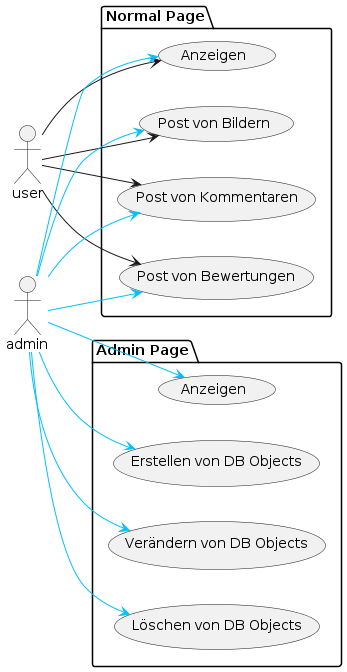
\includegraphics[width=0.45\textwidth]{images/Use Case.png}
    \caption{Use Cases}
    \label{fig:UseCases}
\end{figure}

\newpage

\section{Anforderungen} \label{sec:Anforderungen}
\subsection{Menus} \label{spez:Menus}

Menus sind Objekte, welche in der Datenbank als \code{Menu}-Objekt gespeichert
werden (siehe \ref{fig:DB}, \ref{code:core.models.py}). Jedes \code{Menu} ist
ein Vorkommen eines Gerichts. Um die verschiedenen Vorkommen der
\code{Menu}-Objekte zu gruppieren existiert das \code{MenuType}-Objekt.
Menus mit dem selben Namen wird der gleiche \code{MenuType} zugeordnet.

Die Menus werden von der Mensa-Website gescraped. Die Synchronization (siehe
\ref{spez:Webscraper}) findet bei jedem Aufruf einer der Seiten statt.

Nur wenn das heutige Datum mit dem Datum des Menus übereinstimmt, ist es
möglich, Bilder zu posten (siehe \ref{spez:Images}), das Menu zu bewerten (siehe
\ref{spez:Rating}) und die Posts zu liken (siehe \ref{spez:Liking}).

\subsection{Webscraper} \label{spez:Webscraper}

Der Webscraper ist ein standalone Python Script (siehe
\ref{code:core.webscraper.py}). Der Webscraper stellt mit der Library
\code{requests} Anfragen an die Webseite
\url{https://neuekanti.sv-restaurant.ch/de/menuplan/}. Zuerst werden die Tages-
und Datumsdaten von der Seite geladen. Danach werden die Gerichte (Name,
Beschreibung, Vegan/Vegetarisch) gescraped.

% TODO: Dringens mit den neuen Änderungen umschreiben

Das Script wird bei jedem Aufruf der Webseite ausgeführt. Nach dem Scraping
der Daten werden diese mit der Datenbank (siehe \ref{fig:DB}) verglichen.
Ist das \code{Menu}-Objekt (siehe \ref{spez:Menus}) noch nicht in der Datenbank,
so wird nach einem zugehörigen \code{MenuType} (siehe \ref{spez:Menus})
gesucht. Wenn dieses nicht existiert, dann werden beide Objekte einfach mit den
Daten erstellt. Sonst wird nur das \code{Menu}-Objekt erstellt.

\newpage

\begin{lstlisting}
    data = scrape_data()
    for menu, date in data:
        menus = get_menus_from_db(date=date)
        if menu not in menus:
            menu_type = get_menu_type(menu=menu)
            if menu_type == null:
                menu_type = create_menu_type(menu, data)
            create_menu(data, menu_type)
\end{lstlisting}

(Code in \code{core/webscraper.py})

\subsection{Bilder Gallerie} \label{spez:Gallerie}

Die Bildergallerie ist ein Frontend Feature. Die Bildergallerie wurde von dem
Tutorial auf dieser Seite nachgemacht:
\url{https://www.w3schools.com/howto/howto_js_slideshow.asp}. Die Bildergallerie
wird gebraucht, damit die Images (siehe \ref{spez:Images}) der Menus (siehe
\ref{spez:Menus}) angezeigt werden können.

Im Javascript werden die verschiedenen Bilder in einem Array gespeichert. Nur
das aktive Bild bekommt den style \code{display: block}. Die anderen Bilder
haben \code{display: none}.

Wenn es noch keine Bilder von einem Menu gibt, dann wird ein default Bild
angezeigt.

Da Bilder Hoch- oder Querformat sein können, werden sie auf ihre Orientierung
überprüft. Wenn das Bild Hochformat ist, dann wird es im css anders
behandelt.

\subsection{Posts} \label{spez:Posts}

Der Begriff "Posts" beschreibt zwei verschiedene Objekte in der Datenbank (siehe
\ref{fig:DB}). Es gibt kein übergeordnetes Objekt Posts. Als Posts werden Images
(siehe \ref{spez:Images}) und Reviews (siehe \ref{spez:Reviews}) bezeichnet.

Ein Post, sowie eine Bewertung (siehe \ref{spez:Rating}), kann nur gemacht
werden, wenn das zugehörige \code{Menu} von heute ist. Man kann auch nur die
Posts von dem heutigen Tag liken (siehe \ref{spez:Liking}).

Um einen Post zu schicken, schickt man ein \code{POST-HTML-Form} an das Backend.
Auch im \code{Menu}-View (siehe menu bei {\ref{code:core.views.py}}) wird die
Anfrage verarbeitet. Es wird ausgewertet, was für eine Art Post es ist und es
wird sich dann spezifisch in den \code{post\_function.py} dann um das Speichern
und genauere Auswerten des Formulars gekümmert. Danach wird noch eine
Rückmeldung (\code{message}) an den User gesendet.

\subsubsection{Images} \label{spez:Images}

Es gibt ein \code{Image}-Objekt in der Datenbank (siehe \ref{fig:DB} und in
\ref{code:core.models.py}). Die Image Datei wird nicht in der Datenbank
gespeichert, lediglich eine Referenz, welche auf das Bild verweist.

Wenn das Image auf der öffentlichen Webseite (siehe \ref{spez:Deployment}) angezeigt wird, dann
wird das Image nicht auf dem eigentlichen Server gespeichert, sondern auf einem
Google Drive. Das wird gemacht, da der Server Container keinen persistant
Storage hat.

\subsubsection{Reviews} \label{spez:Reviews}

Es gibt ein \code{Review}-Objekt in der Datenbank (siehe \ref{fig:DB} und in
\ref{code:core.models.py}). Ein Review ist ein Kommentar zu einem Menu
(\ref{spez:Menus}), welcher auf der Webseite angezeigt werden kann.

\subsubsection{Liking} \label{spez:Liking}

Man kann die Posts liken. Dabei wird der Like Counter in der Datenbank (siehe
\ref{fig:DB} und in \ref{code:core.models.py}) erhöht. Ob der User bereits
geliked hat, wird im Javascript Localstorage gespeichert. Die Likes werden nicht
in seperaten Objekten gespeichert, damit die Datenbank nicht zu viele Einträge
bekommt.

Das Liking wird im Javascript gemacht. Die Information wird von dort ins Backend
(siehe like bei \ref{code:core.views.py}) geschickt und dort in der Datenbank
gespeichert. Währenddessen wird der Like Status im Localstorage gespeichert.
Sobald die Anfrage zurückkommt, wird der Like Counter aktualisiert.

\subsection{Rating} \label{spez:Rating}

Ein Rating ist ein Objekt in der Datenbank (siehe \ref{fig:DB} und in
\ref{code:core.models.py}). Ein Rating ist eine Bewertung für ein Menu-Objekt
(siehe \ref{spez:Menus}). Ein Rating hat einen Wert zwischen 1 und 5.

Diese werden auf der Webseite zusammengezählt und der Durchschnitt berechnet,
damit sie auf der Webseite angezeigt werden können.


\subsection{Statistik: Filter und Sortierung} \label{spez:Statistik}

Auflistungen von Menus können gefiltert und sortiert werden. Folgende Filter
können durch einen Button ausgewählt werden: nur vegan, nur vegetarisch und kein
Filter. Folgende Sortierungen können durch einen Button ausgewählt werden:
Rating-Durchschnitt (absteigend), Alphabetisch, Anzahl Ratings und Anzahl
Vorkommen (letzteres nur unter der Seite `alle Menus', weil nur \code{MenuType}
Objekte dieses die Möglichkeit so etwas zu besitzen haben).

Beim Neuladen der Seite werden die Daten aller Menus in der Auflistung aus der
Datenbank gesammelt (bei der Seite `alle Menus' (siehe \ref{code:core.views.py})
werden alle \code{MenuType}-Objekte anstelle der Menus angezeigt) und
standardmässig nach dem Rating-Durchschnitt sortiert. 

Das Filtern und Sortieren auf Knopfdruck erfolgt in Javascript. Die einzelnen
\code{<div>} Elemente im HTML Code, die ein Element der Auflistung beschreiben,
sind standardmässig leer und werden durch die Javascript Funktion
\code{updateListboxs()} mit den Daten der Menus oder MenuTypes gefüllt. Diese Daten sind pro
Menu in einem Javascript Object gespeichert:

\begin{lstlisting}
    menuType = {
        url: data.url,
        name: data.name,
        index: data.index,
        rating: data.rating,
        occurrences: data.occ,
        numrates: data.numrates,
        vegan: data.vegan,
        vegetarian: data.vegetarian,
        visible: true
    }
\end{lstlisting}

(Code in \code{core/templates/allMenu.html})

Je nach Filter wird das visible Attribut auf \code{false} gesetzt, wodurch die
Daten des zugehörigen Menus oder MenuTypes in der Auflistung nicht mehr
angezeigt werden. Das passiert ebenfalls durch die \code{updateListboxs()} Funktion

\newpage

\subsection{Account System} \label{spez:Account}

Die Entwicklung des Accountsystems ist stark von der diesem Django inspiriert
(\url{https://www.youtube.com/playlist?list=PL-osiE80TeTtoQCKZ03TU5fNfx2UY6U4p}).
Allerdings wurde der Code in verschiedenen Projekten bereits verwendet und
dadurch immer weiter entwickelt und vom Tutorial unabhängig gemacht.

Django hat ein eingebautes Accountsystem. Dieses Accountsystem wird in die
Webseite integriert (siehe \ref{code:users.views.py}). Es bietet folgende
Funktionen:
\begin{itemize}
    \item register
    \item login
    \item logout
    \item password-reset
    \item password-reset-done
    \item password-reset-confirm
    \item password-reset-complete
\end{itemize}

Beim Registrieren wird ein \code{User}-Objekt in der Datenbank (noch nicht in der
models.py Datei) erstellt. Danach auch ein \code{Profil}-Objekt (siehe
\ref{code:core.models.py} und \ref{fig:DB}). Beim Registrieren gibt es auch noch
eine ReCaptcha-Überprüfung, damit die Datenbank nicht zugespammt werden kann. Eine Email-Verifikation gibt es nicht

Login und Logout verwalten die Session mit den von Django implementierten
Funktionen.

Die Funktion des Passwordresets funktioniert über die angegebene Email Adresse.
Es wird ein sicherer Token für den Passwordreset an die Email Adresse gesendet.
Die Email wird über einen Gmail Account versendet.

\subsection{Mobile Responsiveness} \label{spez:Mobile}

In Milestone 1 noch nicht implementiert.

\subsection{Punktesystem (Karma)} \label{spez:Karma}

Die Erfahrungspunkte, auch Karma genannt, werden in \code{Profil}-Objekt (siehe
\ref{fig:DB} und \ref{code:core.models.py}) gespeichert.

Man kann Punkte für das Veröffentlichen von Posts (siehe \ref{spez:Posts}) und für
Likes auf den eigenen Posts bekommen. (Funktion \code{add\_karma\_for\_posting})

Mit den Punkten kann man Achievements erreichen (siehe \ref{spez:Badges}).

\subsection{Achievements (Badges)} \label{spez:Badges}

Die Achievements werden als \code{Badge}-Objekt in der Datenbank (siehe \ref{fig:DB} und in
\ref{code:core.models.py}) gespeichert. Die Objekte werden keinem User
zugeordnet gespeichert, sondern dynamisch berechnet, wer welche Achievements
hat.

\begin{lstlisting}
    def get_badges_of_profil(profil):
        badges = Badge.objects.all()

        img_counter = count_best_image_of_profil(profil=profil)
        review_counter = count_best_review_of_profil(profil=profil)
        karma = profil.karma

        categories = [karma, img_counter, review_counter]

        highest_badge = [null, null, null]
        for i in badges:
            if i.count <= categories[i.condition_category]:  # Does the profil own the badge?
                if highest_badge[i.condition_category] is null:
                    highest_badge[i.condition_category] = i
                else:
                    if highest_badge[i.condition_category].count < i.count:
                        highest_badge[i.condition_category] = i
        
        highest_badges = [i for i in highest_badges if i is not None]  # Remove null badges
\end{lstlisting}

(Code in \code{core/statisticFunctions.py})



Es gibt 3 verschiedene Kategorien von Achievements.
\begin{itemize}
    \item Karma-basiert (siehe \ref{spez:Karma})
    \item Images-basiert (siehe \ref{spez:Images})
    \item Review-basiert (siehe \ref{spez:Reviews})
\end{itemize}

Wenn man ein besseres Achievements in einer Kategorie erreicht, dann wird das
alte durch das neue ersetzt. Man kann Achievements auch wieder verlieren, wenn
man die Kriterien nicht mehr erfüllt.

Karma-basiert heisst, man bekommt ein Achievment in dieser Kategorie, wenn man
eine bestimmte Menge an Karma überschritten hat.

Image- und Review-basiert heisst, dass man eine bestimmte Anzahl an `most liked
Images/Reviews' in einem MenuType (siehe \ref{spez:Menus}) hat.

Alle erreichten Achievements sind im Profil ersichtlich (siehe \ref{code:core.views.py})

\subsection{Deployment} \label{spez:Deployment}

Die Webseite wird auf einem Heroku Eco Dyno gehostet. Die Datenbank wird ebenfalls
von Heroku auf einem Postgres Server gehostet. Die Bilder werden auf einem
Google Drive gespeichert (siehe \ref{spez:Images}).

Heroku wurde für dieses Projekt gewählt, weil es eine sehr einfache
\code{Django} Deployment Plattform ist und es sehr viele Anleitung im Internet
gibt. Heroku beitet weiter auch noch viele Addons, welche für
Weiterentwicklungen und Veröffentlichungen nützlich sein könnten. Ausserdem
wurden in vergangenen Projekten gute Erfahrungen mit Heroku gemacht, weswegen
die Wahl auf diesen Anbieter fiel.
